\documentclass[12pt]{article}
\usepackage{graphicx} % Required for inserting images
\usepackage{xcolor}
\usepackage{titlesec}
\usepackage{mdframed}
\usepackage{amsmath}
\usepackage[a4paper,left=22mm,top=20mm,right=22mm]{geometry}
\usepackage{hyperref}
\usepackage{multicol}
\title{Calculus II - Chapter 1 \\   First-order Ordinary Differential Equations }

\author{By Minh Nguyen Quang from USTH Learning Support}
\date{April 2024}
\newmdenv[linecolor=black,skipabove=\topsep,skipbelow=\topsep,
leftmargin=-5pt,rightmargin=-5pt,
innerleftmargin=5pt,innerrightmargin=5pt]{mybox}



\begin{document}

\maketitle
\tableofcontents
\newpage
Why Differential Equations?\\
$\bullet$ One of the oldest subjects in modern mathematics;
\\
$\bullet$ Important role in Engineering, Physics, Life Sciences, Social
Sciences and many areas in mathematical modeling; 
\\
$\bullet$ Newton: study of planetary motion and optics;\\
\begin{center}
    

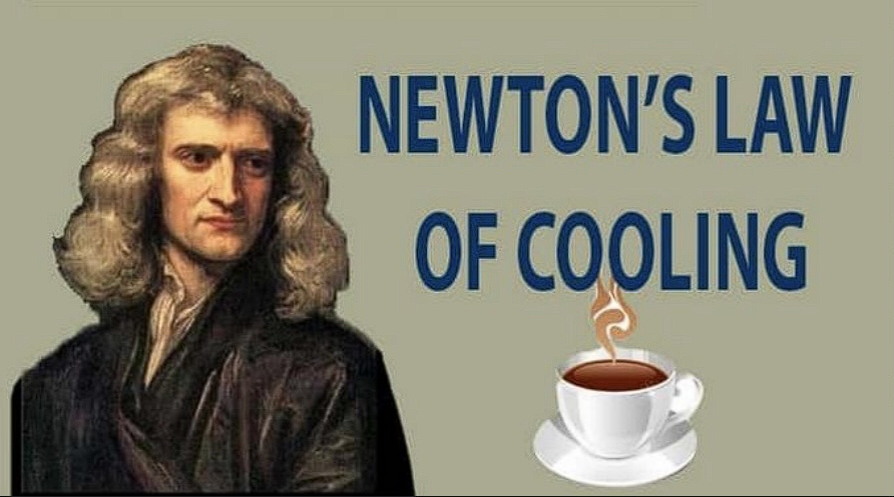
\includegraphics[scale = 0.5]{Ảnh chụp màn hình 2024-06-10 021155.png}
\end{center}
\section{Basic Definition related to Differential Equations}
\subsection{Definition of Differential Equation }
Begin with a very general definition of a differential equation.

\begin{mybox}
    Definition\\ A differential equation is an equation involving one or more
\textcolor{blue}{derivatives} of an unknown function.
\end{mybox}
\begin{mybox}
    Definition:\\ The order of the highest derivative occurring in a differential equation
is called the order of the differential equation. 
\end{mybox}
Example: Define the order of each equation: \\
\\
a) $\frac{dy}{dx} +xy = 0$ 
\\
b) $\frac{d^3 y}{dx^3} + \frac{dy}{dx} = \sin x$
\\
c) $x\frac{d^2 y}{dx^2} + y\frac{dy}{dx} = xy$
\\
d) $ln(\frac{dy}{dx}) + \cos xy = 0$
\newpage
\begin{mybox}
    Any differential equation of order n can be written in the form: 
    $$G(x,y, y',y'',...,y^{(n)}) = 0$$
    where $y^n$ is nth derivative of y respect to x.
\end{mybox}
$\bullet$ In this chapter, we consider first order differential equation.

\subsection{Solution of Differential Equation} 
What is meant by a solution to a differential equation?
\begin{mybox}
    Definition:\\ A function $ y = f(x)$ which is (at least) n times differentiable on an interval I is called a solution to the differential equation
     $$G(x,y, y',y'',...,y^n) = 0$$
     on I, and substitution $y = f(x),y' = f'(x),..., y^{(n)}= f^{(n)}(x)$  reduces
the differential equation to an identity valid for all x $\in$ I. \\
In this case we say that $y = f(x)$satisfies the differential equation.
\end{mybox}
- Solution of differential equation can be in implicit or explicit form. 
\\ 
$\bullet$ Example: Prove that every function in the following family of functions: 
$$y = \frac{1+ ce^t}{1- ce^t}$$
are a solution of differential equation: $y' = \frac{1}{2}(y^2-1)$ \\
Solution: \\
$$y' = \frac{2ce^t}{(1-ce^t)^2}$$
$$\frac{1}{2}(y^2 -1) = \frac{1}{2} (\frac{(1+ce^t)^2}{(1-ce^t)^2} - 1) =\frac{1}{2} \frac{(1+ce^t)^2 - (1-ce^t)^2 }{(1-ce^t)^2} = \frac{1}{2} \frac{4cet^2}{(1-ce^t)^2} = \frac{2ce^t}{(1-ce^t)^2}$$

We see that $y' = \frac{1}{2} (y^2-1)$\\
$\Rightarrow y = \frac{1+ ce^t}{1- ce^t}$ satisfies the differential equation. 
\\
\begin{mybox}
    Definition:\\ A solution to an nth-order differential equation on an interval I is called the general solution on I, if it satisfies the following conditions:\\
    $\bullet$ The solution contains n constants $C_1, C_2, . . . , C_n.$\\
    $\bullet$ All solutions to the differential equation can be obtained by assigning appropriate values to the constants.
\end{mybox}
- Note: Not all differential equations have a general solution.
\\ 
$\bullet$ Example: Find general solution to the differential equation: 
$$y'' = xe^x $$
Solution:\\ 
Integration by part: \\
$$ y' = xe^x - e^x +C_1$$
Integration by part again: \\
$$y = xe^x - 2 e^x +C_1 x+ C_2$$
where C1, C2 are arbitrary constants.

\begin{mybox}
    Definition:\\ A solution to a differential equation is called a \textcolor{red}{particular solution} if it
does not contain any arbitrary constant, except those constants that
already appeared in the differential equation itself.

\end{mybox}
$\bullet$ Example: In previous example, if we assign $C_1 = 0$, $C_2 = 0$ then we have $y = xe^x - 2 e^x$ is a particular solution. \\
\section{Initial Value-Problem}
\begin{mybox}
    Definition:\\ An nth-order differential equation together with n auxiliary conditions of
the form: 
$$y(x_0) = y_0$$
$$y'(x_0) = y_1$$
$$...$$
$$y^{(n-1)}(x_0) = y_{n-1}$$
where $y_0,..,y_{n-1}$ are constants,  is called an \textcolor{purple}{initial-value problem}.
\end{mybox}
$\bullet$ Example: Solve the initial-value problem: \\
$$e^xy' =1$$
$$y(0) = 2$$
Solution: \\
$$\Leftrightarrow y' = \frac{1}{e^x} = e^{-x}$$
$$\Rightarrow y = -e^{-x} + C$$ 
$$y(0) = 2 \Rightarrow C =3 $$ 
Hence $y = e^{-x} +1$ is unique solution. 
\\
\begin{mybox}
    Theorem:\\
    Let $a_1, a_2, . . . , a_n, F$ be functions that are continuous on an interval I. Then, for any $x_0 \in I$, the initial-value problem
    $$y^{(n)} + a_1(x)y^{(n-1)}+...+a_{n-1}(x)y'+ a_n(x)y= F(x)$$
    $$y(x_0)=y_0,y'(x_0) = y_1,...,y^{(n-1)}(x_0)=y_{n-1}$$
    has a \textcolor{red}{unique} solution on I.
\end{mybox}

\begin{mybox}
    Theorem about IVP for first-order differential equation: \\
    \\
    Let's consider the following IVP \\
    $$\frac{dy}{dx} = f(x,y) , y(x_0) = y_0. (1)$$
    If f(x,y) is continuous  in the closed rectangle \\
    $$R = \{(x,y): a \leq x \leq b,c \leq y\leq d\}$$
    and $\frac{\partial f}{\partial y}$ is also continuous in R, then for any interior point $(x_0, y_0)$ in R,
there exists an interval I containing $x_0$ such that the IVP (1) has a
unique solution on I.
\end{mybox}
\section{Separable Differential Equation}
\begin{mybox}
Definition: \\
    A first-order differential equation is called separable if it can be written in the form:
    $$p(y) \frac{dy}{dx}=q(x)$$
    (that is, if we can separate $p(y) dy$ and $q(x) dx)$.
\end{mybox}
$\bullet$ Idea: Group $y$ and $dy$ on one side and $x$ and $dx$ on the other side then take integration two side.  
\begin{mybox}
    Theorem: \\ 
    If $p(y)$ and $q(x)$ are continuous, then Separable Differential Equation has the general solution
    $$\displaystyle \int p(y)dy = \displaystyle \int q(x)dx + C$$
    where C is an arbitrary constant.
\end{mybox}
$\bullet$ Example: Solve this differential equation: \\
 $$1 + x +xy'y = 0$$
 Solution: \\
 Rewrite: \\
 $$1 + x + x \frac{dy}{dx} y = 0$$
 $$\Leftrightarrow y dy= \frac{-1 -x}{x}dx$$
 Integrate two side: \\
 $$\displaystyle \int ydy = \displaystyle \int \frac{-1-x}{x}dx +C$$
 $$\Leftrightarrow \frac{1}{2}y^2 = -ln|x| - x +C$$
 $$\Leftrightarrow y^2 = -2ln|x| -2x +C_1$$
 where C is  an arbitrary constant and $C_1 = 2C$. \\
\\
 $\bullet$ Example: Solve this equation: \\
 $$y' - y^2 -3y + 4 =0$$
 Solution: \\
 - First, note that $y = 1$ and $y = -4$ are solution.\\
 - Next, we consider $y \neq 1$ and $y \neq -4$
 \\
 Rewrite: \\
 $$\frac{dy}{dx} = y^2 +3y - 4  $$
 $$ \Leftrightarrow \frac{1}{y^2 +3y - 4}dy = dx  $$
 $$\Leftrightarrow \frac{1}{(y-1)(y+4)}dy = dx$$
 $$\Leftrightarrow \frac{1}{5}( \frac{1}{y-1} - \frac{1}{y+4})dy = dx$$
 Integrate two side: \\
 $$\displaystyle \int \frac{1}{5}( \frac{1}{y-1} - \frac{1}{y+4})dy = \displaystyle \int dx +C$$
 $$\Leftrightarrow ln|y-1| - ln|y+4| = 5x +5C$$
 $$ \Leftrightarrow ln |\frac{y-1}{y+4}|= 5x +5C$$
 $$\Leftrightarrow \frac{y-1}{y+4} = \pm e^{5x+5C} $$
 $$\Leftrightarrow \frac{y-1}{y+4} = C_1e^{5x} $$
 \\
 where C is an arbitrary constant and $C_1 = \pm e^{5C}(C_1\neq 0)$.\\
 We express y in term of x: \\
 $$y - 1 = C_1e^{5x}(y+4) $$
$$\Leftrightarrow y = \frac{4C_1e^{5x}+1}{1-C_1e^{5x}}$$
Note that, we can not express y = 1 ($C_1 \neq 0$) and y = -4 by above formula. Thus, general solution is: 
$$y = \frac{4C_1e^{5x}+1}{1-C_1e^{5x}} , y = 1,y = -4$$
where $C_1$ is an arbitrary constant.
\section{A simple population model}
We consider model of population growth. 
\\
Let P(t) denote population at time t. We have: 
$$\frac{dP}{dt} = kP$$
where k is positive number.\\
$$\Leftrightarrow \frac{dP}{P}=kdt$$
$$\Leftrightarrow \displaystyle \int \frac{dP}{P}= \displaystyle \int kdt + C$$
$$\Leftrightarrow lnP = kt +C$$
(P is greater than 0) \\
$$\Leftrightarrow P = e^{kt +C}$$
$$\Leftrightarrow P = P_0e^{kt}$$
where $P_0 = e^C$. 
\\
\begin{mybox}
    Definition: \\
    1. The formula above is called the Malthusian growth model.\\
    2. The time taken for such a culture to double in size is called the
\textcolor{red}{doubling time}.
\end{mybox}

$\bullet$ Example: According to the data listed at www.census.gov, the world’s population reached 6 billion persons in mid-1999, and was at that time increasing at a rate of about 212,000 persons each day. Assume that the natural population growth at this rate continues, that t = 0 corresponds to mid-1999, and that 1 year = 365.25 days. Use the natural growth equation P’ = kP to find:\\
(a) the annual growth rate, correct to 4 decimal places.\\
(b) the world population by mid-2017 to the nearest million\\
(c) How long it will take, to the nearest year, for the world’s population to reach 60 billion which is what some demographers believe is the maximum population that the planet can support. In what year will the population reach 60 billion?\\
Solution: \\

a)\\
We have: \\
$$\frac{dP}{dt}= kP$$ $$\Rightarrow k = \frac{dP}{dt} \div P = \frac{212000}{6 \times 10^9} = 3.53 \times10^{-5}$$
b)\\
$P_0=6\times 10^9$\\
$t = (2017 -1999) \times 365.25 = 6574.5$ (days)
\\
$$P = P_0e^{kt} = 7.567 \times 10^9$$
c) \\
Apply formula, we have: \\
$$60 \times 10^9 = 6 \times 10^9 e^{kt}$$
$$ t = 65230  \text{ days} \approx 178.6 \text{ years} $$

\section{First-Order Linear Differential Equation }
$\bullet$ Recall: \\
\textcolor{pink}{Linear Equation}: \\
1.  Linear equations have no products or roots of variables and
 no variables involved in trigonometric, exponential, or logarithmic functions.
\\
2. Variables appear only to the first power \\
\begin{mybox}
    Definition of Linear Differential Equation: \\
    A differential equation that can be written in the form:
    $$a_0(x)y^{(n)} + a_1(x)y^{(n-1)}+...+a_{n-1}(x)y'+ a_n(x)y= F(x)$$
    where $a_0,a_1,...,a_n,F$ are function of x only, is called Linear Differential Equation of order n. \\
    Such a differential equation is linear in $y,y',..,y^{(n)}$. 
\end{mybox}
$\bullet$ Example: \\
(1) $yy' = 2x^2$: not linear \\
(2) $2xy + 3xy' = 5x$: linear\\
\newpage
\begin{mybox}
    Definition of First-order Linear Differential Equation: \\
    A differential equation that can be written in the form:
    $$a(x)\frac{dy}{dx} +b(x)y =r(x)$$
    where $a(x),b(x),r(x)$  are functions defined on an interval (a, b), is called a \textcolor{blue}{ first-order linear differential equation}.
\end{mybox}
$\bullet$ Idea: Try to make form derivative of product (uv)' = u'v +v'u. \\
\\
\textcolor{red}{Technique to solve First-Order Linear Differential Equation}

\begin{mybox}
    Step 1: Assume that $a(x) \neq 0$, divide both side by $a(x)$ to make \textcolor{blue}{standard form}: 
    $$ \frac{dy}{dx} +p(x)y = q(x)$$
    where $p(x) = \frac{b(x)}{a(x)}$ and $q(x) = \frac{r(x)}{a(x)}$\\
    \\
    Step 2: Multiply two side by $e^{ \int p(x)dx}$ (integrating factor) \\
    $$e^{ \int p(x)dx} \frac{dy}{dx} +p(x)e^{ \int p(x)dx}y = e^{\int p(x)dx}q(x)$$
   $$\Leftrightarrow (e^{ \int p(x)dx} y)' = e^{ \int p(x)dx}q(x) $$
   Step 3: Integrate two side: \\
   $$\Leftrightarrow e^{ \int p(x)dx} y = \int{(e^{ \int p(x)dx}q(x) )dx} + C $$
   $$\Leftrightarrow y = \frac{1}{e^{ \int p(x)dx}} (\int{(e^{ \int p(x)dx}q(x))dx} + C) $$
\end{mybox}

$\bullet$ Example: Solve Differential Equation: \\
$$y' - 2xy =  -2x^3$$
Solution: \\
Integrating factor: $e^{\int -2x} = e^{-x^2}$
$$e^{-x^2}y'-2xe^{-x^2}y = e^{-x^2}(  -2x^3)$$
$$\Leftrightarrow (e^{-x^2}y)' =  e^{-x^2}(  -2x^3)$$
$$\Leftrightarrow e^{-x^2}y =  \int (  e^{-x^2}(  -2x^3))dx +C$$
We consider $I = \int (  e^{-x^2}(  -2x^3))dx $.\\
Use Integration by part, we have: 
$$ u = x^2 \Rightarrow du = 2xdx$$
$$dv = -2xe^{-x^2}dx \Rightarrow v= e^{-x^2} $$
$$\Rightarrow I = x^2e^{-x^2} - \int e^{-x^2}2xdx = x^2e^{-x^2}+ e^{-x^2}$$
$$\Rightarrow e^{-x^2}y =x^2e^{-x^2}+ e^{-x^2} +C $$
$$\Leftrightarrow y = x^2 +\frac{C}{e^{-x^2}}+1 = x^2 +Ce^{x^2}+1$$
Solution is $y = x^2 +Ce^{x^2}+1 $, where C is an arbitrary constant. 
\\
\\
$\bullet$ Example: Solve Differential Equation:\\
$$ y' +y\cos x = \sin x\cos x$$
Solution: 
\\
Integrating factor: $e^{\int \cos x} = e^{\sin x}$
$$\rightarrow e^{\sin x}y'+ \cos x e^{\sin x}y = e^{\sin x}\sin x\cos x$$
$$\Leftrightarrow (e^{\sin x}y)' = e^{\sin x}\sin x\cos x $$
$$\Leftrightarrow e^{\sin x}y = \int e^{\sin x}\sin x\cos x dx +C$$
$$\Rightarrow e^{\sin x}y = \sin xe^{\sin x} - e^{\sin x} +C$$
$$\Rightarrow y = \sin x -1 + \frac{C}{e^{\sin x}}$$
\\
where C is an arbitrary constant. 
\\
\section{Change of Variables}
\subsection{Homogeneous of degree zero}
\begin{mybox}
    A function $f(x, y)$ is said to be homogeneous of degree zero if
    $$f(tx,ty) = f(x,y)$$
    for all positive values of t for which $(tx, ty)$ is in the domain of f.\\
    Equivalently, $f$ is homogeneous of degree zero if it is invariant under a re-scaling of the variables x and y.

\end{mybox}
$\bullet$ Example: Determine whether the given function is homogeneous of degree zero: \\
a) $\displaystyle f(x,y) = \frac{x^2-y^2}{xy}$
\\
b)$\displaystyle f(x,y) = \frac{x}{xy+1}$\\
\\
c) $\displaystyle f(x,y) = \frac{x+y}{x^3 +1}$\\
\\
Solution: \\
a) $\displaystyle f(tx,ty) = \frac{t^2x^2-t^2y^2}{t^2xy} = f(x,y)$ \\
b) $\displaystyle f(tx,ty) = \frac{tx}{t^2xy+1} \neq f(x,y)$\\
c)$\displaystyle f(tx,ty) = \frac{t(x+y)}{t^3x^3+1} \neq f(x,y)$
\\
\\
$\bullet$ We can write function $f(x,y)$ in term of $\frac{x}{y}$ or $\frac{y}{x}$. 
\begin{mybox}
    Theorem: \\
    A function $f(x, y)$ is homogeneous of degree zero if and only if it
depends on either $\frac{x}{y}$ or $\frac{y}{x}$ only. 
\end{mybox}

\subsection{Homogeneous first-order differential equations}

\begin{mybox}
    Definition: \\
    If $f(x, y)$ is homogeneous of degree zero, then the differential equation
    $$\frac{dy}{dx} = f(x,y)$$
    is called a homogeneous first-order differential equation.
\end{mybox}
- To solve homogeneous differential equation, we can rewrite function $f(x,y)$ into $F(\frac{y}{x})$ and let $V(x) = \frac{y}{x}$ \\
\\
\textcolor{red}{Technique to solve Homogeneous first-order differential equations}\\
\begin{mybox}
    $$\frac{dy}{dx} = F(\frac{y}{x}), xV(x) =y $$
    Step 1: Express $\frac{dy}{dx}$ by $\frac{dV}{dx}$ \\
    $$\frac{dy}{dx} = V + x\frac{dV}{dx}$$
    Step 2: Substitute\\ 
    $$V + x\frac{dV}{dx} = F(V)$$
    Step 3: Using technique to solve Separable Differential Equation: \\
    $$\frac{1}{F(V) -V}dV = \frac{1}{x}dx$$
\end{mybox}
- Note: We can see that, by using change variable xV(x) = y, we can reduce s a homogeneous first-order differential equation to Separable Differential Equation: \\
$\bullet$ Example: Solve Differential Equation: \\
$$y' =\frac{x}{y}+ \frac{y}{x} +1$$
Solution: 
\\ 
Let $V(x) = \frac{y}{x}$: 
$$\Rightarrow V + x\frac{dV}{dx} = \frac{1}{V} + V +1 $$
$$\Leftrightarrow x\frac{dV}{dx} = \frac{V+1}{V}$$
$$\Leftrightarrow \frac{V}{V+1}dV=\frac{1}{x}dx$$
$$\Leftrightarrow (1 - \frac{1}{V+1})dV = \frac{1}{x}dx$$
Integrate two side: 
\\
$$\int (1 - \frac{1}{V+1})dV = \int\frac{1}{x}dx +C $$
$$\Leftrightarrow V - ln|V+1| = ln|x| +C $$ 
$$\Leftrightarrow \frac{y}{x} - ln|\frac{y}{x} +1| =ln|x| +C$$
$$\Leftrightarrow \frac{y}{x} - ln|y+x| =C$$
where C is an arbitrary constant. 
\\
\subsection{Bernoulli Equations}
We now consider a special type of nonlinear differential equation that
can be reduced to a linear equation by a change of variables. 
\begin{mybox}
    Definition: \\
    A differential equation that can be written in the form: 
    $$\frac{dy}{dx} +p(x)y = q(x)y^\alpha (*)$$ 
    where $\alpha$ is a real constant, is called \textcolor{red}{Bernoulli Equation}.
\end{mybox}
$\bullet$ If $\alpha$ = 0 or 1, equation (*) is first- order linear differential equation.  \\
\\
$\bullet$ Example: 
\\
a)  $\displaystyle \frac{dy}{dx}+x^2y = (x^4+x^3)y^2$
\\
b) $\displaystyle \frac{dx}{dy} +y^3x = ln(y)x^2$
\\
\newpage
\textcolor{pink}{Technique to solve Bernoulli Equation}\\

\begin{mybox}
     $$\frac{dy}{dx} +p(x)y = q(x)y^\alpha (*)$$ 
     Step 1: Divide two side by $y^\alpha$
     $$y^{-\alpha}\frac{dy}{dx} + y^{1-\alpha}p(x) = q(x)$$
     Step 2: Let $u(x) = y^{1-\alpha}$ 
     $$\frac{du}{dx} =(1-\alpha) y^{-\alpha}\frac{dy}{dx}$$
     Step 3: Substitution 
     $$\frac{1}{1-\alpha} \frac{du}{dx} + up(x) =q(x)$$
     \\
     Step 4: Solve First - Order Linear Equation

    
\end{mybox}
$\bullet$ Example: Solve Differential Equation: \\
$$y' -y = -y^2$$
Solution: 
\\
- First, y = 0 is solution. \\
- Next, we consider $y \neq 0$\\
$$\Leftrightarrow y^{-2}y' - y^{-1} = -1$$
Let u = $y^{-1}$
$$\frac{du}{dx} = -y^{-2}\frac{dy}{dx}$$
$$\Rightarrow -\frac{du}{dx} -u = -1$$
$$\Leftrightarrow \frac{du}{dx} + u =1$$
Multiply two side by $e^x$: 
\\
$$e^x\frac{du}{dx} + e^xu = e^x$$
$$\Leftrightarrow (e^xu)' = e^x$$
$$\Leftrightarrow e^xu = \int e^xdx + C$$
$$\Leftrightarrow u = \frac{C}{e^x} + 1$$
$$\Rightarrow y^{-1} = \frac{C}{e^x} + 1$$
$$\Rightarrow y = \frac{e^x}{e^x + C}$$
Solution of this differential equation are $y = \frac{e^x}{e^x + C}$ and $y = 0$,
where C is an arbitrary constant. \\
\\
$\bullet$ Example: Solve Differential Equation \\
$$x^2y'+2xy = y^3$$
Solution: \\
First, y = 0 is a solution. \\
Next, we consider $y \neq 0$
$$\frac{x^2}{y^3}y' + \frac{2x}{y^2} = 1$$
$$\Leftrightarrow y^{-3}y'+ \frac{2}{x}y^{-2} = \frac{1}{x^2}$$
Let $u = y^{-2}$
$$\frac{du}{dx} = -2y^{-3}\frac{dy}{dx}$$
$$\Rightarrow \frac{-1}{2}\frac{du}{dx} + \frac{2}{x}u = \frac{1}{x^2}$$
Standard Form: \\
$$\frac{du}{dx} - \frac{4}{x} u = \frac{-2}{x^2}$$
Multiply both side by $x^{-4}$: 
$$ x^{-4} \frac{du}{dx} -4x^{-5}u = -2x^{-6}$$
$$\Leftrightarrow (x^{-4}u)' = -2x^{-6}$$
$$\Leftrightarrow x^{-4}u = \int -2x^{-6}dx + C$$
$$ \Leftrightarrow x^{-4}u = \frac{2
}{5}x^{-5} + C$$
$$\Leftrightarrow u = \frac{2}{5} x^{-1} + Cx^{4}$$
$$\Rightarrow y^{-2} =\frac{2}{5} x^{-1} + Cx^{4}$$
$$y^2 = \frac{1}{\frac{2}{5} x^{-1} + Cx^{4}}$$
Solution of this differential equation are $y^2 = \frac{1}{\frac{2}{5} x^{-1} + Cx^{4}}$ or $y =0$, where C is an arbitrary constant. 
\\
\section{Exact Differential Equations}
The technique presented in this section is for first-order differential
equations written in a differential form:\\
$$M(x,y)dx + N(x,y)dy = 0(*)$$
$\bullet$ If we have u =(x,y), u is function of two variable x and y, y is function of variable x. Then differential du is defined by: 
$$du = \frac{\partial u}{\partial x}dx + \frac{\partial u}{\partial y}dy$$
$\bullet$ Idea: Try to transform (*) into derivative of u(x,y)\\
\begin{mybox}
    Definition:  \\
    The differential equation\\
    $$M(x,y)dx + N(x,y)dy = 0(*)$$
    is said to be exact in a domain D of the xy-plane if there exists a
function $u(x, y)$ such that: \\
$$\frac{\partial u}{\partial x} = M,\frac{\partial u}{\partial y} =N$$
for all $(x,y) \in D$. 
\end{mybox}
The function $u(x,y)$ called a \textcolor{red}{potential function}for the differential
equation.
\\

\textcolor{blue}{$\bullet$ Solution technique for exact d.e. }

\begin{mybox}
    Theorem: \\
    The general solution to an exact differential equation:
     $$M(x,y)dx + N(x,y)dy = 0(*)$$
     is defined implicitly by:
     $$u(x,y) =C$$
     where C is an arbitrary constant and $u(x, y)$ is determined by
integrating the system:
 $$\frac{\partial u}{\partial x} = M,\frac{\partial u}{\partial y} =N$$
 
\end{mybox}
\textcolor{red}{$\bullet$ Test for exactness}
\\
\newpage 
\begin{mybox}
    Theorem: \\
    Let D be a simply connected domain in the xy -plane. Then the differential equation
     $$M(x,y)dx + N(x,y)dy = 0(*)$$
     is exact for all $(x, y) \in  D$ if and only if
     $$\frac{\partial M}{\partial y} = \frac{\partial N}{\partial x} $$
\end{mybox}
$\bullet$ Example: Solve Differential Equation
\\
$$(3x^2+6xy^2)dx + (6x^2y+ 4y^3)dy = 0$$
Solution: 
\\
Check for Exactness: 
$$\frac{\partial M}{\partial y} = \frac{\partial N}{\partial x} = 12xy$$
$\rightarrow$  Exact differential equation. There exists a
potential function u such that
$$\begin{cases}
    \frac{\partial u}{\partial x} = 3x^2+6xy^2  (1) \\
    \frac{\partial u}{\partial y} = 6x^2y+ 4y^3 (2)
  \end{cases}$$
From (1), we integrate w.r.t x, keep y as fixed: 
$$u(x,y) = x^3 + 3x^2y^2 +g(y)$$
where $g(y)$ is an arbitrary function of y.
\\
Derivative function u above w.r.t y: 
\\
$$\frac{\partial u}{\partial y}=6x^2y +\frac{dg}{dy}(3)$$
From (2) and (3), we have: 

$$\begin{cases}
    \frac{\partial u}{\partial y}=6x^2y +\frac{dg}{dy}(3) \\
    \frac{\partial u}{\partial y} = 6x^2y+ 4y^3 (2)
  \end{cases}$$
$$\Rightarrow \frac{dg}{dy} = 4y^3$$
$$\Leftrightarrow g(y) = y^4$$
$\rightarrow$ Solution of exact differential equation is: 
$$ u(x,y) = x^3 + 3x^2y^2 + y^4 = C $$
where C is an arbitrary constant. 
\section{Numerical Solution to First-order Differential Equations}
Our final approach to analyzing first-order differential equations is to
look at the possibility of constructing a numerical approximation to the
unique solution to the initial-value problem: 
$$\frac{dy}{dx} = f(x,y), y(x_0) =y_0$$
The idea is to generate a sequence of approximations $y_1, y_2, . . .$ to the
value of the exact solution at the points $x_1, x_2, . . .,$ where $x_{n+1} = x_n + h$
n = 1, 2, . . ., and h is a real number.\\ 
\\
$\bullet$ Remark: \\
- Numerical methods don’t generate a formula for the solution to
differential equation. 
\\
- Rather they generate a sequence of approximations to the values
of the solution at specific points.\\
\\
\textcolor{blue}{$\bullet$} \textcolor{red}{Euler's Method} 
\\
 We have IVP: 
$$\frac{dy}{dx} = f(x,y), y(x_0) =y_0$$
First, suppose we wish to approximate the solution to the IVP at
$x = x1 = x0 + h$, where h is small.
\\
We write tangent equation pass through $(x_0,y_0)$:
$$y = y_0 + \frac{dy}{dx}(x-x_0)$$
Because we have $\frac{dy}{dx}=f(x,y)$ and consider $\frac{dy}{dx}$ at first point $(x_0,y_0)$, tangent line: 
$$y = y_0 + f(x_0,y_0)(x-x_0)$$
Setting $x = x_1$ in the last equation yields the so-called Euler
approximation to the exact solution at $x_1$ 
$$y_1 = y_0 + f(x_0,y_0)(x_1-x_0)$$
$h = x_1 -x_0$ 
$$\rightarrow y_1 = y_0 + hf(x_0,y_0)$$
Continuing this process, we can determine the sequence of
approximations
$$y_{n+1}=y_n + hf(x_n,y_n)$$
\\
$\bullet$ Example: Use Euler's Method with step size = 0.5 to compute the
 approximate y-values $y_3$ of solution of the initial-value problem:
 $$\frac{dy}{dx} = y - 2x, y(1) =0$$
 Solution: \\
 $$x_0 = 1, y_0 =0$$
 $$y_1 =y_0 +hf(x_0,y_0) = 0 + 0.5f(1,0) = -1$$
 $$x_1 =1.5 , y_1 = -1$$
 $$y_2 = y_1 + hf(x_1,y_1) = -1 + 0.5f(1.5,-1) = -3$$
 $$x_2 = 2, y_2 = -3$$
 $$y_3 = y_2 +hf(x_2,y_2) = -3 + 0.5f(2,-3) = -6.5$$
 \newpage
 \section{Exercises}
 Solve First- Order Differential Equation.
 
 \begin{multicols}{2}
\begin{enumerate}
    \item[1.] \( y' =x^2y \)
    \item[2.] \( (2xy +3)dy = -y^2dx \)
    \item[3.] \( xy' + y = \sqrt{x} \)
    \item[4.]\(ydx+(x+x^2y^2)dy=0\)
    \item[5.]\((x+2y)dx-xdy=0\) 
    \item[6.]\(y' =\displaystyle \frac{x+y-2}{x-y+4}\) 
    \item[7.]\((x^2y^2-x)dy=ydx\)
    \item[8.]\(xy'+y=-xy^2\) 
\end{enumerate}
\end{multicols}

\begin{center}
    “When you really want something the whole universe conspires in helping you to achieve it” \\
(The Alchemist, Paulo Coelho)
\end{center}
  
  \newpage
\begin{center}
    \textbf{FEEDBACK FOR THIS DOCUMENT}\\
    
\includegraphics[width=0.5\linewidth]{qr.jpg}\\
    \textbf{Please scan this QR code...}\\
    \textbf{Or click this link:} \url{https://forms.gle/qmMhmKmVWHVKNAaG6} \\
    to give us feedback on this document!!!
\end{center}
Please spend a little time to send your feedback. Although it is just a simple work, it has great significance to us. Your feedback can help us improve our future documents and it let us know whether you understand what we have written in this document. Thank you so much for using our documents!\\
\begin{center}
    Good luck with your exam!
\end{center}

\end{document}
